%%%%%%%%%%%%%%%%%%%%%%%%%%%%%%%%%%%%%%%%%
% Thesis
% LaTeX Template
% Version 1.2 (29/7/12)
%
% This template has been downloaded from:
% http://www.latextemplates.com
%
% Original authors:
% Steven Gunn
% http://users.ecs.soton.ac.uk/srg/softwaretools/document/templates/
% and
% Sunil Patel
% http://www.sunilpatel.co.uk/thesis-template/
%
% License:
% CC BY-NC-SA 3.0 (http://creativecommons.org/licenses/by-nc-sa/3.0/)
%
% Note:
% Make sure to edit document variables in the Thesis.cls file
%
%%%%%%%%%%%%%%%%%%%%%%%%%%%%%%%%%%%%%%%%%

%----------------------------------------------------------------------------------------
%	PACKAGES AND OTHER DOCUMENT CONFIGURATIONS
%----------------------------------------------------------------------------------------
%!TEX encoding = UTF-8 Unicode
\documentclass[11pt, a4paper, oneside]{Thesis} % Paper size, default font size and one-sided paper
\usepackage[T1]{fontenc}
\usepackage[utf8]{inputenc}
\DeclareUnicodeCharacter{00A0}{~}
\graphicspath{{./Figures/}} % Specifies the directory where pictures are stored

\usepackage[square, comma, sort&compress]{natbib} % Use the natbib reference package - read up on this to edit the reference style; if you want text (e.g. Smith et al., 2012) for the in-text references (instead of numbers), remove 'numbers'

% Packages for use with nomenclature
\usepackage[intoc]{nomencl}
\makenomenclature
%\renewcommand{\nomname}{List of Abbreviations}
\usepackage{mfirstuc} % Added for function which makes the first character of a word upper case
\newcommand*{\nom}[2]{#1\nomenclature{\makefirstuc{#1}}{#2}}

\newcommand*{\fig}[2]{
	\begin{figure}[th]
	    \begin{center}
    	    \includegraphics[width=0.60\textwidth]{#1.png}
	        \caption{#2}
        	\label{#1}
    	\end{center}
	\end{figure}
}

\usepackage{listings}
\usepackage{color}
\definecolor{lightgray}{rgb}{.9,.9,.9}
\definecolor{darkgray}{rgb}{.4,.4,.4}
\definecolor{purple}{rgb}{0.65, 0.12, 0.82}

\lstdefinelanguage{JavaScript}{
  keywords={typeof, new, true, false, catch, function, return, null, catch, switch, var, if, in, while, do, else, case, break},
  keywordstyle=\color{blue}\bfseries,
  ndkeywords={class, export, boolean, throw, implements, import, this},
  ndkeywordstyle=\color{darkgray}\bfseries,
  identifierstyle=\color{black},
  sensitive=false,
  comment=[l]{//},
  morecomment=[s]{/*}{*/},
  commentstyle=\color{purple}\ttfamily,
  stringstyle=\color{red}\ttfamily,
  morestring=[b]',
  morestring=[b]"
}

\lstset{
   language=JavaScript,
   backgroundcolor=\color{lightgray},
   extendedchars=true,
   basicstyle=\footnotesize\ttfamily,
   showstringspaces=false,
   showspaces=false,
   numbers=left,
   numberstyle=\footnotesize,
   numbersep=9pt,
   tabsize=2,
   breaklines=true,
   showtabs=false,
   captionpos=b
}

%\hypersetup{hidelinks=true} % Go to http://en.wikibooks.org/wiki/LaTeX/Hyperlinks for information about configuration
\title{\ttitle} % Defines the thesis title - don't touch this
\def\theartefact{madame}
\def\Theartefact{Madame}
\def\THEARTEFACT{MADAME}
\def\website{\url{http://madame.elseth.me}}
\begin{document}

\frontmatter % Use roman page numbering style (i, ii, iii, iv...) for the pre-content pages

\setstretch{1.5} % Line spacing of 1.3

% Define the page headers using the FancyHdr package and set up for one-sided printing
\fancyhead{} % Clears all page headers and footers
\rhead{\thepage} % Sets the right side header to show the page number
\lhead{} % Clears the left side page header

\pagestyle{fancy} % Finally, use the "fancy" page style to implement the FancyHdr headers

\newcommand{\HRule}{\rule{\linewidth}{0.5mm}} % New command to make the lines in the title page

% PDF meta-data
\hypersetup{pdftitle={\ttitle}}
\hypersetup{pdfsubject=\subjectname}
\hypersetup{pdfauthor=\authornames}
\hypersetup{pdfkeywords=\keywordnames}

%----------------------------------------------------------------------------------------
%	TITLE PAGE
%----------------------------------------------------------------------------------------

\begin{titlepage}
\begin{center}

\includegraphics[width=8cm]{Figures/uib-emblem-svart} \\[0.5cm]
% 
\includegraphics{uib-emblem-svart}\vfill % University/department logo - uncomment to place it
\textsc{\LARGE \univname}\\[1.5cm] % University name
\textsc{\Large Master Thesis}\\[0.5cm] % Thesis type

\HRule \\[0.4cm] % Horizontal line
{\huge \bfseries \ttitle}\\[0.4cm] % Thesis title
\HRule \\[1.5cm] % Horizontal line

\begin{minipage}{0.4\textwidth}
\begin{flushleft} \large
\emph{Author:}\\
\href{http://blog.elseth.me}{\authornames} % Author name - remove the \href bracket to remove the link
\end{flushleft}
\end{minipage}
\begin{minipage}{0.4\textwidth}
\begin{flushright} \large
\emph{Supervisor:} \\
{\supname} % Supervisor name - remove the \href bracket to remove the link
\end{flushright}
\end{minipage}\\[2cm]

% \large \textit{A thesis submitted in fulfilment of the requirements\\ for the degree of \degreename}\\[0.3cm] % University requirement text
\textit{in the}\\[0.1cm]
\groupname\\\deptname\\[0.5cm] % Research group name and department name

{\large \today}\\[1cm] % Date
\end{center}

\end{titlepage}

%----------------------------------------------------------------------------------------
%	QUOTATION PAGE
%----------------------------------------------------------------------------------------

\pagestyle{empty} % No headers or footers for the following pages

\null\vfill % Add some space to move the quote down the page a bit

\textit{``It depends upon what the meaning of the word 'is' is"}

\begin{flushright}
-- Bill Clinton
\end{flushright}

\vfill\vfill\vfill\vfill\vfill\vfill\null % Add some space at the bottom to position the quote just right

\clearpage % Start a new page

%----------------------------------------------------------------------------------------
%	ABSTRACT PAGE
%----------------------------------------------------------------------------------------

\addtotoc{Abstract} % Add the "Abstract" page entry to the Contents

\abstract{\addtocontents{toc}{\vspace{1em}} % Add a gap in the Contents, for aesthetics
In this thesis I will describe the methods used in creating the artefact: \theartefact\ \Theartefact\ \THEARTEFACT\
}

\clearpage % Start a new page

%----------------------------------------------------------------------------------------
%	ACKNOWLEDGEMENTS
%----------------------------------------------------------------------------------------

\setstretch{1.5} % Reset the line-spacing to 1.3 for body text (if it has changed)

\acknowledgements{\addtocontents{toc}{\vspace{1em}} % Add a gap in the Contents, for aesthetics
TODO
}
\clearpage % Start a new page

%----------------------------------------------------------------------------------------
%	LIST OF CONTENTS/FIGURES/TABLES/NOMENCLATURES PAGES
%----------------------------------------------------------------------------------------

\pagestyle{fancy} % The page style headers have been "empty" all this time, now use the "fancy" headers as defined before to bring them back

\lhead{\emph{Contents}} % Set the left side page header to "Contents"
\tableofcontents % Write out the Table of Contents

\lhead{\emph{List of Figures}} % Set the left side page header to "List of Figures"
\listoffigures % Write out the List of Figures

\lhead{\emph{List of Tables}} % Set the left side page header to "List of Tables"
\listoftables % Write out the List of Tables

\lstlistoflistings

\printnomenclature[5em] % Print the page header and list of nomenclature

%----------------------------------------------------------------------------------------
%	DEDICATION
%----------------------------------------------------------------------------------------

% \setstretch{1.5} % Return the line spacing back to 1.3

% \pagestyle{empty} % Page style needs to be empty for this page

% \dedicatory{For/Dedicated to/To my\ldots} % Dedication text

% \addtocontents{toc}{\vspace{2em}} % Add a gap in the Contents, for aesthetics

%----------------------------------------------------------------------------------------
%	THESIS CONTENT - CHAPTERS
%----------------------------------------------------------------------------------------

\mainmatter % Begin numeric (1,2,3...) page numbering

\pagestyle{fancy} % Return the page headers back to the "fancy" style

% Include the chapters of the thesis as separate files from the Chapters folder
% Uncomment the lines as you write the chapters

% Chapter Template

\chapter{Introduction} % Main chapter title

\label{Introduction}
%use \ref{Introduction}

\lhead{Chapter \ref{Introduction}. \emph{Introduction}} % Change X to a consecutive number; this is for the header on each page - perhaps a shortened title

%----------------------------------------------------------------------------------------
%	SECTION 1: Background
%----------------------------------------------------------------------------------------

% \section{Background} Should this be used as the main introduction before the motivation? ala Aleksander Larsen
The Internet is now an ingrained part of our everyday life,
and the amount of content and services that are available through it is growing at an ever increasing rate.
For all this information to be of use to humans it is necessary to have some interface through which to access the parts of it that are relevant to us.
\citet{Shirky2007} tells of the early attempts to structure the Web,
using ontologies and hierarchies created by experts.
This soon got clunky as the number of documents increased,
and this way of organizing information fell out of favor to be replaced by searching for information using keywords.
It is this phase of organizing information we are in now.

\citet{Berners-Lee2001} suggested that we could do better than keyword matching.
With searching as it works today users have to manually check the results from the search engine,
and compare the results from several documents, following links as is necessary.
Instead of forcing users to go through this process,
this new idea was to enrich the documents we put on the Web with metadata that could be read and reasoned about by computers.
By doing this we could move the tedious task of siphoning though Web sites looking for relevant information from users
over to specialized software agents that could collect information on the topic and return the answer to the user.

This does create some extra work for content creators on the Internet.
Adding metadata to content is not a trivial task.
The W3C recommends using RDFa to add metadata \citep{Pemberton:08:RXS}.
But to use RDFa the user not only needs to know the syntax of RDFa itself,
but also which ontologies exists that contain the meaning the creator wants to convey,
and knowledge about how those ontologies are structured to use them in the correct way.

Ontology is the philosophical discipline of finding out which things exist,
the manner in which one can say that these exist and how these can be categorized.
When talking about ontologies in the context of the Semantic Web,
an ontology can be explained as a collection of things that one can describe using the ontology,
and how these things can relate to each other.

%----------------------------------------------------------------------------------------
%	SECTION 2: Motivation
%----------------------------------------------------------------------------------------

\section{Motivation}
According to \citet{Gantz2011} the amount of information in the world now doubles every two years.
Should this trend continue, we are going to need better ways of searching through all the information that is generated.
We are going to need to be able to search for content in a way that lets us search for concepts, not only keywords.
What we want is to have linked semantic data that help move the burden of finding relevant content from us over to machines.

At the moment, adding semantic markup to Web sites is unfeasible for most content creators on the Web.
Adding proper metadata does not only mean that you need to know HTML,
but also that you need to understand the concept of ontologies, and know of the different ontologies that exist.
In addition you need to know of the implementation of \nom{RDFa}{Resource Description Framework in attributes}, microdata or microformats
as well as the content of the specific ontologies you intent to use on your site.

Adding metadata shouldn't really be that hard.
Humans are good at knowing what things are.
We know what the things on Web sites mean, and which concepts they are meant to convey.
Natural language is mainly ambiguous to computers, not human beings.
I want to create a tool that lets users use their knowledge of natural language and the concepts it conveys
to create metadata by disambiguating the language for the computer, and letting it create the mappings and the elements on the Web page.

The aim of this thesis will be to develop a prototype artefact that will let users add metadata to Web pages using natural language.
The prototype should map to the schema.org ontology,
as using this ontology can increase the visibility of the Web page in search results in the most popular search engines.
The tool should also be able to express meaning in other ontologies, so that it can help create a rich Web of interconnected data.

The prototype tool will be created using Node.js\footnote{\url{http://nodejs.org}},
a JavaScript platform based on Google Chromes JavaScript runtime,
and using MongoDB\footnote{\url{http://www.mongodb.org}} as a database solution.
JavaScript is a good language to rapidly create prototypes, and the flexibility and simplicity inherent in using the same language
server side, client side and in database communication, inspired me to try using and learning these tools for the thesis.

%It is estimated that the amount of information created by humans before 2005,
%
%is smaller that the amount of information created after 2005.

I choose to develop using node.js because it's a new and exciting technology that would make it possible to write
the entire app using one programming language for front-end, server side and as the database query language.

Creating a Web application allows the work to consist both of back end server side components, and front-end work.

%----------------------------------------------------------------------------------------
%	SECTION 3: Research Questions
%----------------------------------------------------------------------------------------

\section{Research question}
The main research question in this thesis is:

\emph{"Is it possible to create a tool which allows naïve users to easily add metadata to their Web sites using natural language?"}

In this context we should understand "naïve users" as users who do not have any training in the use of semantic technologies,
and who do not have any knowledge about the ontologies used for testing in this thesis.

To answer this question I will develop a tool called \theartefact, a play on the goal "MetADAta MAde Easy".
The tool will consist of a logical backend tied to a Web front-end,
and the different modules will be created in an iterative way to get working proofs of concepts for testing early.

There are several sub questions that will need to examined to answer this question.
\begin{itemize}
	\item How should users pick the parts of a Web page they want to add metadata to, and find the concepts it describes using natural language?
	\item Is WordNet suitable for representing disambiguated concepts from natural language in a way that will allow us to map these concepts to formal ontologies?
	\item How should an algorithm be implement to finds mappings from the natural language concept to types in
			formal ontologies in a way that preserves the semantic content of the concept?
	\item Is it possible to add metadata to Web pages in such a way that it does not change the way the page is rendered by browsers?
\end{itemize}

In addition I will also need to solve the technical problems of how to import and export Web pages from the artefact,
and how to save the resulting documents on the server.

\section{Target audience}
The main goal of the work with \theartefact\ is to lower the barrier of entry for enhancing Web sites with metadata.
I want to make metadata accessible to content creators on the Web that do not know enough about Semantic Web technologies
to add this data them selves.

Due to availability of English natural language resources this thesis will focus development on mapping English text,
and limit the target group to users who write content in English.
I will also assume that the users control the HTML of their Web pages,
and that being provided with a new HTML document will allow the user to update their documents.


% Chapter Template

\chapter{Theory} % Main chapter title

\label{Theory} % Change X to a consecutive number; for referencing this chapter elsewhere, use \ref{ChapterX}

\lhead{Chapter \ref{Theory}. \emph{Theory}} % Change X to a consecutive number; this is for the header on each page - perhaps a shortened title

\section{Ontology and folksonomy}
One of the central concepts in semantic web technology is that of the ontology. 
In philosophy Ontology is the branch dealing with the study of which things 'exists', and if it is possible to categorize these things. 
For artificial intelligence \citet{Gruber1993} explained it as "an explicit specification of a conceptualization". 
That is than one commits to a given conceptualization of the domain in question, and formalize how we describe and reason about these conceptualizations. 
\citet{Pretorius2004} also gives a good overview of the history of the term, and show several of the interpretations and formalisms. 
One can also go to \citet{Noy1997} to find comparisons of several of the early ontologies, including WordNet which will be important in this thesis.

\citet{Shirky2007} criticizes the use of ontologies as a way of trying to enforce a structure on something that is by nature unstructured. 
He instead pushes the idea of common tagging. 
Part of the reason he criticizes the ontology approach is that it seem improbable that experts can know the needs of all the users a priori, and therefor that every ontology will prove to be inadequate.
%\citet{Doan2002} Tror ikke denne skal brukes
On the semantic web, ontologies are represented using collection of RDF( Resource Description Framework) triplets. 
These triplets are in the form of <subject, predicate, object>, much like simple declarative sentences \citep{Berners-Lee2001}. 
Each subject and predicate, and some objects, is represented by an URI( Universal Resource Identifier), which links to the resource that describes it.

While ontologies are formally constructed taxonomies, folksonomies are informal taxonomies generated by collecting tags or annotations from collaborative tagging systems on a given platform\citep{Tang2009}. 
\citet{Mika2005} has given a more formal definition of folksonomy where he sees a folksonomy as a set of tags T, 
$T \subseteq A \times C \times I$, where A is the set of users tagging, C is the set of tags, and I is the set of objects being tagged.
\citet{Gruber2007} suggested that one should add the source of the tag, and some kind of rating system to help filter out junk tags. 
\citet{Scerri2008} on the other hand suggests removing the objects being tagged from the ontology, 
seeing that the objects that are being described are not part of the tool to describe them.
Instead they like Gruber want to add the source of the tag, the number or times a tag occur, and the tagging behavior of each user.
\citet{Bang2008} explains the difference between ontologies and folksonomies by classifying them as a priori and a posteriori annotations. 
That is, ontologies are created by experts as ways on conceptualizing a domain, folksonomies on the other hand are samples of how people speak or think about a domain.
Folksonomies grew as a subject of research as it became popular for users to tag content on the internet with keywords they felt were relevant.

For users tags are convenient, since Adding additional tags can make it easier for humans to search and browse collections. This is especially true for multimedia content, which we don't yet have good tools for searching in \citep{Weinberger2008}.
Tags provide meta data about content in a way that makes sense to humans. From an information retrieval perspective this is interesting since it means that humans in some way add meaning to the content.
There however are several problems with using tags as the basis of a semantic web. \citet{Tang2009} mention several. 
Tags are supposed to be written in natural language, and natural language has words that are synonymes(words that are written in different ways, 
but mean the same), homonymes(words with different meanings that are written in the same way), or polynyms( a word that can have several meanings) 
making it unsuitable for computer reasoning since they are ambiguous \citep{Passant2008}. 
As \citet{Golder2005} mentions, users also operate on different levels of abstraction, which can make it harder to find interesting resources.
In addition to this comes the problem of non dictionary words, both new, or compound words, or simply words that have been misspelled\citep{Tonkin2006}.


There has been done a lot of research into how one can lift semantic data out of these unstructured tags.
\citet{Golder2005} has done research into the statistical analysis of tags. 
The analysis done here show that there seems to develop vocabularies of frequently used tags. 
This might help diminish the effect of misspelled and nonsense words. Similar findings were also reported by \citep{Shirky2007}

There has also been done research into automatic clustering. 
\citet{Mika2005} created clusters by creating weighted graphs, and compared using tag concurrence and actor interest as weights.  
\citet{Brooks2006} has done work an categorizing blogs entries by tags, to see if concurrence of tags indicated similar content. 
Using the most common tags did give some results, but only broad categories. The results were not better than extracting words that were given asserted to be relevant for the category.

\citep{Tang2009} tries to go further that clustering tags, and tries to build an hierarchical model from a folksonomy. 
They use a probabilistic model that takes into account the frequency and concurrence of tags and tries to generalize it to an ontology. 
The method does get good results in creating the hierarchy, but does also show som inappropriate sub/super category inferences.

\citet{Weinberger2008} suggests a method for removing ambiguity from tags,
 by suggesting additional tags to the user when the tag entered can belong to one of several distinct sets 

While there are many difficulties attached to merging the social and semantic web, and with lifting semantic data from tags, there are many researchers who stress the need for this \citep{Passant2007,Mika2005, Gruber2007}.

\section{WordNet and lexitags}
\label{TheoryWordNet}
Lexitags \citep{Veres2011} utilizes a different approach for getting semantic meaning out of tags that the approaches mentioned until now. 
Instead of analyzing existing folksonomies and try to lift semantic data out of these tags, the idea presented is to turn it around and make users attach meaning to the tags at input time.
This is done by letting users disambiguate the tags by using WordNet synsets, an idea that was also mentioned by.

WordNet is a lexical reference system that stores words in sets of synonymes called synsets. The idea is to separate the word form from the word sense. 
The underlying assumption is that the user already knows English, is familiar with the concepts that are conveyed, 
and doesn't need definitions to understand, but can use synonymes to identify the meaning they want to convey\citep{Miller1990}.

In addition to storing these synsets WordNet also contains information about the semantic relationship between different concepts. 
The synonymy relationship is obviously contained within each synset, 
though it should be mentioned that the definition used in WordNet is not one where substitution never changes the truth value of a sentence. 
WordNet uses a weaker definition where two word forms can be seen as synonymes in relation to some semantic context. 
The antonymy relationship is another relationship between word forms. While the exact definition of antonymy is hard to pin down, the intuitive notion that an antonym to x is not-x will take us a long way\citep{Miller1990}.

WordNet also stores information about hyponymy and hypernymy, which is a relationship between concepts.
 A hypernym can be explained as a generalization of some concept, a hyponym on the other hand can be seen as a specialization of a concept. 
 \{tree\} can for example be seen as a hyponym of \{plant\}, and the reverse relation is a hypernymy relation \citep{Veres2010}.

The fact that WordNet separates sense and form is good for our purposes, as we are interested in the sense, not the form of the word. 
Mapping tags to synsets removes the ambiguity that arrises from multiple spellings. 
At the same time, since the mapping preserves the form of the tag this can still be kept for analysis if one finds that there are significant differences in how different forms of a synset is used\citep{Veres2011}.
By enforcing this mapping to WordNet lexitags also gets access to the hierarchical knowledge therein, and can create lightweight ontologies by using hypernyms of the tags as SuperTags, a method introduced by \citet{Veres2010}.
The mapping to WordNet also add some perks. There is a mapping between WordNet and Schema.org\footnote{\url{https://github.com/mhausenblas/schema-org-rdf}}, and between WordNet and the SUMO( Suggested Upper Merged Ontology)\citep{Niles2003}.

Using WordNet to ground the semantics of the tags was idea also suggested by \citet{Cattuto2008}. But \citet{Cattuto2008} suggested using a post hoc analysis of the tags in a social network, instead of enforcing the mapping though an interface.

One critique of WordNet comes from \citet{Mika2005} who points out that while WordNet can catch lexical sameness, it lacks cultural awareness. The example used was that of the tie between Noah and the ark.
This tie would be obvious for most humans, and would most lightly be caught through clustering tags, but would not be caught by WordNet.

\citet{Passant2008} has also suggested a system where taggs are disambiguated by the user at input time. A difference between the systems is that Passant and Laublet suggested using URIs to online resources for disambiguation.

\section{WordNet}
In a written dictionary the most efficient way to organize data is to list the words alphabetically, 
since the act of finding words is the most labor intensive part.
As long as the dictionary is tied to an analog form it is hard to structure the content otherwise as it would make
finding words to difficult. 
With the advent of computer dictionaries, the act of looking up words is no longer time consuming or difficult, 
and the posibility to experiment with new structures for the dictionary became possible.

There are several differences between ordinary dictionaries and WordNet. 
The motivation behind WordNet was to create a dictionary that categorized words by the concepts they represented.
To accomplish this the structure was based on earlier psycholexicologic research\citep{Miller1990}.
 
One of the ways this psycholexicological background comes to sight is in that WordNet separates words into four syntactical categories: nouns, verbs, adjectives and adverbs\citep{Miller1995}.
This was based in part on work done by \citet{Fillenbaum1965} which showed that participants would most frequently 
assosiate words with other words from the same syntactical category.

This way of categorizing the words is able to take advantage of the fact that the different syntactical categories have different semantic structures.
In this thesis we will use the noun category of WordNet, and benefit from it's topoligical hierarchy.
For completeness we'll also mention that verbs are organized as entailment relations, 
while adjectives and adverbs are organized as N-dimentional hyperspaces\citep{Miller1990}.

The word 'word' is ambigious as it can be used to describe the representation of a word, and its underlying semantics.
Natural language is built on conventions that tie together utterances or symbols, with some thing or idea.
A symbol or utterance is the form of a word, while the thing or idea it represents is the words meaning.
We can represent this idea using Table \ref{table:LexicalMatrix}( see page \pageref{table:LexicalMatrix}).
The table shows a lexical matrix, which means to make explisit the relation between form $F$ and meaning $M$.
The forms and meanings are linked using entries $E_{(x,y)}$ which would state that meaning $M_x$ has the form $F_y$.
It also shows how both a single form can refere to several meanings, 
and how a single meaning can be represented using several forms.
Within the categories mentioned WordNet then tries to organize the words not by form, 
but by similarity of meaning.

This organisation is done by grouping words which are synonymes into sets. 
We will describe these sets of synonymes( synsets), by enclosing one or more word forms in curly brackets.
We could for example use the synset \{dog, domestic dog, Canis familiaris\} to describe the common dog. 
When precision is not the point we will use a short form like \{dog\} to describe the same meaning.
To organize words into synsets in this way ont first needs to have a clear idea about what one means by synonymy.
A strict definition of synonymy would claim that for form $F$ and $F'$ to be synonymous one must be able
to replace one with the other in any sentence without changing the truth value of that sentence.
This is similar to using Leibniz law of identity to qualify synonymy.
WordNet uses a weaker definition where one says that whether two forms are synonymes is dependent on the 
semantic context that they are inn, and that two words can be synonymes with respect to this semantic context\citep{Miller1990}.
This weaker definition still necessitates that words must be from the same syntactic category to be synonymous, 
and explains together with \citet{Fillenbaum1965} why it's useful to separate the syntactic categories.

\begin{table}[h]
	\centering
	\begin{tabular}{|c||ccccccc|}
		\hline
	        Word     & 	~		 & ~		 & Word Forms & ~ & ~ & ~ & ~		  \\ 
	        Meanings & F$_1$     & F$_2$     & F$_3$      & . & . & . & F$_n$     \\ \hline
	        M$_1$    & E$_{1,1}$ & E$_{1,2}$ & ~          & ~ & ~ & ~ & ~         \\ 
	        M$_2$    & ~         & E$_{2,2}$ & ~          & ~ & ~ & ~ & ~         \\ 
	        M$_3$    & ~         & ~         & E$_{3,3}$  & ~ & ~ & ~ & ~         \\ 
	        .        & ~         & ~         & ~          & . & ~ & ~ & ~         \\ 
	        .        & ~         & ~         & ~          & ~ & . & ~ & ~         \\ 
	        .        & ~         & ~         & ~          & ~ & ~ & . & ~         \\  
	        M$_m$    & ~         & ~         & ~          & ~ & ~ & ~ & E$_{m,n}$ \\
		\hline
	\end{tabular}
	\caption{A lexical matrix showing the relation between the forms and meanings of words, from \citet{Miller1990}}
	\label{table:LexicalMatrix}
\end{table}


\subsection{Hyponymy and hypernymy}
Hyponymy and hypernymy is the main way that nouns are organized in WordNet.
Hypo- and hypernymy are a different type of relation between words than synonymy.
While synonymy is a relation between different forms of a word, 
hypo- and hypernymy are relations between word meanings.
The two are the inverse relation of each other and we will explain them by defining what makes something a hypernym.
The concept $M$ is the hypernym of some other concept $M'$ if $M$ is such that native speakers of English would agree
with claims of the type "$M'$ is a type of $M$". 
As an example: \{animal\} would be a hypernym of \{dog\}, 
since a native user of English would agree that "a dog is a type of animal".
Hypernymy is transitive, meaning that if $M$ is a hypernym of $M'$, and $M'$ is a hypernym of $M''$, 
then $M$ is a hypernym of $M''$.
So since we know that dog is a type of animal, and that labrador is a type of dog, 
we also know that \{animal\} is a hypernym of \{labrador\}.
In addition to being transitive, hypernymy is also asymmetric.
This means that the fact that $M$ is a hypernym of $M'$ entails that $M'$ cannot be a hypernym of $M$.
When we know that \{animal\} is the hypernym of \{labrador\}, 
we also know that \{labrador\} is not a hypernym of \{animal\}\citep{Miller1990}.

Hyponymy is the inverse relation of hypernymy. 
This means that if $M$ is a hypernym of $M'$, then $M'$ is a hyponym of $M$. 
The fact that \{animal\} is a hypernym of \{labrador\} means that \{labrador\} is a hyponym of \{animal\}.
Hyponymy is also transitive and asymmetric\citep{Miller1990}.

Another aspect of this relation with respect to nouns is the fact that one asserts some type of inherence from the more
general hypernyms to its more specialized hyponyms. 
This means that if one knows that a concept has some properties, 
then the hyponymes of that concept will have all the same properties, 
in addition to the properties it has which distinguishes it from the concept\citep{Miller1990a}.
This has some basis in psycholexicologic research. 
\citet{Collins1969} showed that subjects used less time to say that a concept inhabited some property when that property
was viewed as more typical for concept, than if it were a property of some more general concept
( see Figure \ref{MemoryStructure}, page \pageref{MemoryStructure}).
A subject would for example use less time establishing that a shark is dangerous, a property associated with sharks;
than they would establishing that it had fins, a property associated with fish; or that it breaths, associated with animals( see Figure \ref{MemoryStructure}, page \pageref{MemoryStructure}).

Nouns in WordNet is organized in a hierarchal fashion. 
One organizational issue then is if one should organize the nouns as one, or several hierarchies.
WordNet started by organizing the nouns into 25 semantic prime categories.
When these had been created one realized that these contained natural groupings.
At this point one decided to add some top level synsets which tied these together, 
with the most general being \{entity\}\citep{Miller1990a}.

\begin{figure}[h]
    \begin{center}
        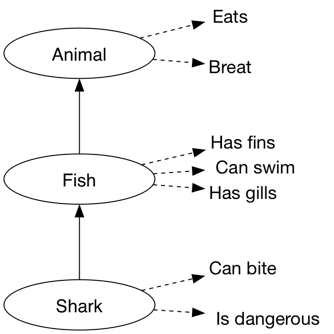
\includegraphics[width=0.60\textwidth]{MemoryStructure.png}
        \caption{A hypothetical memory structure, from \protect \citet{Collins1969}}
        \label{MemoryStructure}
    \end{center}
\end{figure}

% Chapter Template

\chapter{Methodology} % Main chapter title

\label{Methodology} % Change X to a consecutive number; for referencing this chapter elsewhere, use \ref{ChapterX}

\lhead{Chapter \ref{Methodology}. \emph{Methodology}} % Change X to a consecutive number; this is for the header on each page - perhaps a shortened title

The thesis utilizes the design research methodology to perform its research.
I will use the guidelines provided in \citet{Hevner2004} to ensure that the process is rigorous.
The guidelines provided in this article are:
\begin{enumerate}
	\item \label{gl1}Design as an Artifact
	\item \label{gl2}Problem Relevance
	\item \label{gl3}Design Evaluation
	\item \label{gl4}Research Contributions
	\item \label{gl5}Research Rigor
	\item \label{gl6}Design as a Search Process
	\item \label{gl7}Communication of Research
\end{enumerate}

I will now explain how I intend to follow these guidelines for the work related to this thesis.
The first guideline says that a design research project should produce some artefact.
Designing an artefact is central to this thesis.
I will use the system \theartefact\ to test my research question,
and the success of the system will decide whether the research question can be answered positively.

In the introduction I described my motivation for the thesis, and why it is a relevant contribution to design science.
I described the need for computer readable metadata for information retrieval,
and the difficultly inherent in the creation of this data for new users.
The work performed in completing this thesis can help lower the barrier of entry for generating semantically enriched websites.
If successful I hope to that the results can be used to both increase the value of computer search in general,
and increase the visibility and discoverability of the webpages that use tools that build on the work done.

Design evaluation is also mentioned and this guideline stresses the need for rigorous evaluation of the artefact that has been developed.
To evaluate the success of the project I will look at the artefacts ability to map natural language to ontologies.
The goal is to generate metadata that is of the level of quality as existing metadata of a comparable type.
I will also examine if it can add the metadata to the webpage using RDFa, without changing the way the webpage is rendered by browsers.

The main research contribution of this project will be \theartefact\,
which will contribute to solve the problem of how to get users to create semantic content.
This prototype system can serve, either as a starting point for development,
or as an inspiration as to how one can create a system that makes it easier to create semantic content on the web.

The need for research rigor, which is mentioned in guideline \ref{gl5} will be followed by following the multimethodological approach suggested in \citet{Chen1990} and \citet{NunamakerJr1990}.
\fig{MultiMethodological}{{A multimethodological approach to IS research, from \protect \citet{Chen1990}}}
\citet{Chen1990} proposes four activities for the design process that interact in the development of information systems
(see figure \ref{MultiMethodological} on page \pageref{MultiMethodological}).
The paper suggests using a multimethodological approach where one moves between different research activities:
Theory building, experimentation, observation and systems development.
By using these different approaches I hope that I will be able catch important facets that might otherwise have been missed or over looked.

Guideline \ref{gl6} says that design research should be a search process.
In this context that means that one should explore the possible implementations of the artefact by iterating through phases of
generating prototypes and testing these prototypes against the requirements of the project (as seen in figure \ref{GenerateTestCycle},
page \pageref{GenerateTestCycle}).
To attain this type of cycle I choose to use a system development methodology that utilizes multiple iterations of building and testing.

The last guideline proposed has to do with clear communication of the results of the research.
It is further proposed that one should take care to have several channels of communication with different levels of technical detail.
The reasoning is that one needs to convince both the technical and the managerial communities.

To conform to the seventh guideline one should communicate the results of ones research in such a way that it is accessible for the intended target audience.
The primary way of communicating the research will be this thesis.
The thesis will target an academic audience and describe the process of development,
and the evaluation of the artefact.

In addition the work done on the project is made available to the developer community,
with hopes that others can build on the work done in relation to this thesis.
All the source code from the project is open source,
developed and shared on GitHub\footnote{The project can be found at: \url{https://github.com/EivindEE/Madame}},
and released under the MIT license.
Releasing the source code of the project means that others can learn from the system in another way than what they
could just by reading this theses, as most of the details of implementation are outside the scope of an academic thesis.
It also means that all those who wish to improve upon the work,
either by resolving issues with the codebase or by adding new features,
can do so in a way that can enrich the tool for all those who wish to use it.

\fig{GenerateTestCycle}{{The generate/test cycle, from \protect \citet{Hevner2004}}}



% Chapter Template

\chapter{Design and Development} % Main chapter title

\label{DesignAndDevelopment} % Change X to a consecutive number; for referencing this chapter elsewhere, use \ref{ChapterX}

\lhead{Chapter \ref{DesignAndDevelopment}. \emph{Design and Development}} % Change X to a consecutive number; this is for the header on each page - perhaps a shortened title

%----------------------------------------------------------------------------------------
%	SECTION 1
%----------------------------------------------------------------------------------------

Describe the process of development,
and which parts of \theartefact\ which were developed during the different stages of development.
We are then going to give a high level overview of the system.
After giving an outline of the development process and the system,
the main parts of the system will be described in greater detail.

\section{The different phases of development}
We will now describe the different phases of development.
This will outline the main sequence in which work on \theartefact\ was done.
This overview of the iterations will explain when the initial development of
the different part were to give an short explanation of the development process.

\subsection{Iteration 1}
The first iteration started with a technical peak exploring different tools and frameworks for development with javascript.
We wanted to find tools that could reduce development time by reducing the amount of repetitive work done in the project.

It was decided that we were going to use bootstrap\footnote{\url{http://twitter.github.io/bootstrap/}} as a grid system
for the webpage.
Using a standard grid system makes it easier to create a webpage that looks OK,
and reduces the amount of time needed to set up a scaffold.
Since the visual aspect of the webpage was not an important aspect of the work a simple grid system like bootstrap
eased the development burden.

We also decided to use SASS\footnote{\url{http://sass-lang.com}} to write our stylesheets.
The syntax is similar to that of CSS.
We decided to use this instead of CSS since it contained variables,
making it posible to make global changes while only modifying one line in the stylesheet.
SASS compiles to standard CSS.

JavascriptSince javascript lacks a good IDE we wanted to have some tool that would check our code to make sure that the
code was consistent and that the syntax was correct.
We decided to use jslint\footnote{\url{http://www.jslint.com}} to validate our code.
Using a linter eases development as it enforces a particular coding standard for the project.
The way the project was set up, we couldn't build the project without it passing the linting test.

Since the project depended on compiling the stylesheet and linting the code we decided to use grunt.js\footnote{\url{http://gruntjs.com}}
to automate this process.
Grunt.js is a task manager that can run certain tasks when specified events are triggered.
We set the project up so that each time a javascript or SASS file was saved we compiled the SASS document,
and concatenated the public javascript files.
Concatenating the javascript files meant that we didn't have to update the HTML when we created or deleted a new
javascript file, since we only needed to include that one file.

We had decided to use Node.js as the development platform of the project.
Setting up a basic server in node.js can be done in a single line of code,
but requires a lot of low level handeling of requests and responses
including parsing request url to find the correct handler.
We decided to instead go for express\footnote{\url{http://expressjs.com}},
a web app framework which simplifies routing requests to the correct handler and handeling static files.
It was also decided to use the jade\footnote{\url{http://jade-lang.com}}
templating language to generate the HTML that was used on the website.
Using a templating language made the distinction between structure and content clearer,
and enabled reuse of structure and content between different versions of the website during development.

Our technological peak also included geting to know the DOM, the API used for manipulating HTML documents.
The problem we tried to solve during this technical peak was how to find minimal legal ranges.
We knew we were going to have to add separate tags to add the metadata we create,
and that we were going to let users select which portions of the text that carried the semantic content.
Since the user selection might not be a legal HTML range we worked on an algorithm to find the smallest range that
was both a legal range, and which contained the whole of the selected text.


\subsection{Iteration 2}
The next step consisted of actually generating metadata tags with the correct RDFa syntax which enclosed the user selection.
One of the tasks was giving each selected section a unique id so that they could be referenced externaly,
we also wanted this id to carry some information about the content of the tag.
At this stage we had not yet started with development of the mapping so the tags contained mock data.

In this iteration we also started work with generating the hypernym chains we needed to find mappings.
We initially tried to use an existing triple store and query the information with SPARQL.
The triple store used an early version of SPARQL which did not allow recursive queries.
Since we needed to find the transitive closure of the hypernym relation,
using this source would require multiple sequencial queries and would take to long to be tenable.
Javascript does not have a mature library for querying the WordNet database, so we did not have a native solution.
Our solution was instead to use perl to write a script which could query a local WordNet instance.
This again required a technical peak to learn the basics of the perl programming language but gave a satisfying solution.

We also used this iteration to find WordNet mapping files and convert them to a format more suitable for our system.
We had a mapping file between WordNet and SUMO in the WordNet database format,
and one between WordNet and schema.org in RDF.
Both of these files were translated into javascript objects.

\subsection{Iteration 3}
In the third iteration we implemented the actual mapping algorithms that we wanted to try out.
We implemented one that starts with looking at all the hypernyms of the synset,
and one that looks alternately at hypernyms and siblings.

This was also the iteration where we created a mechanism for fetching HTML from other websites so that they could be
marked up using \theartefact.

\subsection{Iteration 4}
In the fourth iteration we made the export module.
This module would take the webpage that the user had imported into the system and create a new HTML document.
This document would be stored in our database, and would be accessible for the user through a URL which we provided when the page was exported.

Adding properties to entities was also developed during this stage.
This was only implemented for schema.org properties,
both to keep the number of properties at a managable level,
and because extracting all the allowed properties for all SUMO classes would be a difficult task.

In this iteration we also added the ability to add author information.
This is not closely tied to the problem of translating natural language to formal ontologies,
but it is tied to allowing users to add metadata in a simple way without knowing about the formal underpinnings.

\subsection{Iteration 5}
The last iteration consisted of testing and refactoring the system.
We wrote some test scripts that would run the best fit algorithms we had created over a set of synsets,
and print out the resulting mappings along with information about whether the algorithms gave corresponding results,
and the measure of quality of the mapping.
The results of these tests will be discussed further in section \ref{ComparingAlgorithms}.

\subsection{Overview completed system}
The artefact was divided into several modules which function independently of each other.
The modules were loosely coupled so that each module could be changed or modified without affecting the other modules.
The modules that were created were:
\begin{itemize}
	\item The web front end
	\item A module that fetched and processed the HTML from the sites that the user wanted to mark up
	\item A module for fetching possible disambiguating terms from lexitags
	\item A module for finding the best fit mappings for SUMO and schema.org
	\item A module for finding the best fit mappings from DBPedia to schema.org
	\item A module that puts the document back in its initial state and saves it to a persisten storage
\end{itemize}

\section{Interaction method}
\label{Interaction}
When we first faced the problem of how to let users interact with the web app we thought that using the highlighting or
selection of text to be the most intuitive approach.
We also believed that this would be the simplest interaction method to implement.
The simple case of taking selected text and displaying it in the console can be implemented as in listing \ref{DOMSelection}.

\begin{lstlisting}[caption={Logging selected text}, label=DOMSelection]
	var logSelection = function () {
		console.log(window.getSelection().getRangeAt(0).toString());
	};
	document.addEventListener('mouseup', logSelection);
\end{lstlisting}

The "mouseup" event is triggered every time the user has pressed and then released the mouse pointer on the website.
This event is not available on mobile and tablet type browsers,
but adding listeners for corresponding events should not be difficult if we later see the need for this.

In the web app the selected text is sent to the web server to find possible disambiguations for the text.
The lexitags service that we use for disambiguation now is targeted towards disambiguating single words.
It does handle some composite terms and some proper nouns, but this is outside the normal use case.
The lexitags service is designed to disambiguate single tags, not large paragraphs of text.
To accommodate this we do a simple check for the length of the text string.
If the length of the string is more than the longest allowed length,
the query is instead replaced with a shorter query indicating that the selection is of a larger section of text.

The response from the server is a JSON string containing the terms that were found to be possible senses of the selected text.
Each of these senses have an explanation property which gives a short textual description of the meaning of the sense.
These senses are displayed as a list on the web site.
The senses that are returned come from different sources.
They can come either from WordNet and take the form of WordNet synsets, or they can be resources from DBPedia.
Both of these can be used to generate mappings,
but the most interesting mapping for this thesis lies in generating mappings from WordNet so the synsets are given preference in the list.
DBPedia does not have a standardized way of finding the super type of a resource,
so if the resource does not have a schema.org mapping it is difficult to find generalizations that do.
Lexitags also returns the top level resources from schema.org as shown in figure \ref{TopLevelSchemaOrg}(page \pageref{TopLevelSchemaOrg}).
These are sorted to the bottom of the list as these are fallbacks for when none of the of the terms suggested for
the word turn out to be reasonable suggestions for the selected text.

\subsection{Adding types}

To select one of the terms from the list as the meaning of the selected text the user clicks the sense in the list see in
figure \ref{SidebarMeanings}.
\fig{SidebarMeanings}{The list of posible interpretations of "discoveries"} % IMAGE OF LIST OF INTERPRETATIONS
When a sense is clicked it is sent to the server to be mapped.
The servers uses the best fit algorithm described in \ref{BestFitMapping}(page \pageref{BestFitMapping}) to find the ontology references
that fits the sense best and attaches these references to the selection using RDFa.
The algorithm used to attach the metadata to the selection can handle an arbitrary amount of namespaces and references.
If there is duplication of references these will be dropped.

When the metadata element is created,
the schema.org type is sent back to the server to get a list of the possible properties of that type.
On the server we use a JSON representation of the schema.org ontology to find the properties that a type can have.
The representation we use was retrieved from \url{http://schema.rdfs.org} which is a support site that tries to
promote linked data.
For each of the types in schema.org the JSON file provides the properties specific to that type,
and all the properties it has inherited from its super types.
We combine the information about which properties a type can have with a short description of what the property represents,
and information about the range of the property, that is the range of values that are valid values of the property.
The resulting JSON object is then returned to the website.
These properties are then added to the metadata element as separate elements,
with the description and range stored as data attributes of the element.

\subsection{Adding properties}

Users can click text that has been tagged with metadata.
This triggers a popover view which displays the properties that the element can have,
and which types of values are allowed for each property as shown in figure \ref{PropertiesFull}.
\fig{PropertiesFull}{{The properties popover for schema:Event}} % IMAGE OF PROPERTY SELECTION BOX
If the property allows other schema.org types as their value we do a scan of the content of the website to check if
there are elements of the correct type on the page.
Elements of the correct type that are found are put in a combo box and can be selected as values for the property.
In all cases the user is presented with the option of writing the value of the property in an input field.
If the property already has a value it will be displayed in the input field when the popover is displayed.

%\fig{Sidebar}{The information tab of the sidebar},

\section{Maintaining the well-formedness of the document}
One of the difficult aspects of adding the metadata to the selections was making sure that the HTML was well-formed
after the metadata was inserted.

Special care needs to be taken with the ranges of the selection.
Since we need to insert the metadata into tags we can't just use the user range without some checks.
If we consider the simple case:

\texttt{<p>some text \hl{in a p</p> <p>` pluss some} other text </p>}

If we simply inserted a tag we would get invalid HTML since we would have overlapping elements.

\texttt{<p>`some text <tag> in a p</p> <p> pluss some </tag>  other text </p>}

To get a well formed HTML document we need to either close and open the HTML tags

\texttt{<p>some text </p><tag><p> in a p</p> <p> pluss some </p></tag><p>  other text </p>}

Solving the problem in this manner would change the structure and rendering of the webpage,
as we would create new block elements.
This is not a tenable solution as we want to leave the page looking the same as we found it.
Our solution would instead expand the range of the selection so that it covered a larger part of the document:

\texttt{<tag><p>some text in a p</p> <p> pluss some other text </p></tag>}

The interaction method consists of letting the user make arbitrary selections and then adding metadata to the selection.
This could easily lead to overlapping elements in the HTML as shown above.
To avoid this malformed HTML we check the range of the selected text and see if surrounding it with a tag
containing metadata would result in a well-formed document, and modify the range if needed.
If the start and end of the selection are in the same element then adding metadata is safe.
If that is not the case we find the smallest change we need to make to the scope of the range to make it safe.
There are two general cases her, when either the start or the end of the range is in a descendant element of the other,
and when both start and end are descendants of a common element but not of each other.

In the first case we need to find out which element is the descendant of which.
We do that by following the ancestor links of each element.
When we find that either the start or end element has the other as an ancestor we use the ancestor which is the direct
child of the other element and place the start or end tag right before or after that tag, depending on which element
descended from which.

When the elements are not descendants of each other we know that they must be descendants of some other element.
If nothing else they must both be descendants of the root element.
We use a similar approach for this case as we do for the fist,
but instead of finding the ancestor which is the direct child of the other node we find the one which is a child of the
closest common node.
We then surround these elements with the metadata tag.
This metadata element is styled with a distinct color to let the user know that the text is tagged.

\section{Importing webpages}
One of the issues that came up early was how to import and display the websites that the user wanted to add metadata to.
Early attempts tried using the iframe\footnote{http://www.w3.org/TR/html5/embedded-content-0.html\#the-iframe-element}
element of \nom{HTML}{HyperText Markup Language}.
Embedding the target website in an iframe was the first try as it would allow the page to display in the same maner
as it does when accessed directly.
Using the iframe element in this maner would however constitute cross-domain communication and is not allowed.
The solution that is used in the system now uses a module on the server to fetch the HTML of the document the user wants to enrich.
The HTML that is imported is now appended to a content element in the webapp.
We attach the javascript events used in the webapp to this element,
to keep the interaction confined to the content the user is meant to tag.
We also use the id of this tag to tell if a certain element is a part of the user content section by checking if it is
the child of the element.

The user writes the URL of the webpage into an input field on the top of the webapp as shown in figure \ref{MadameHeader}.
\fig{MadameHeader}{The header of the \theartefact\ webapp} % IMAGE OF THE HEADER OF MADAME
The server will fetch the document stored at that location.
We created a proxy to get the html from other websites.
The proxy would take a URL and get the resource located there.
If the resource is not of the right type i.e. not a HTML document with a body element,
the proxy would return an error.
When the resource has been downloaded the content of the body element of the document is parsed to comment out code that
could be harmful, that could make the page display incorrectly, or that could disrupt the way the webapp functions.
The parts of the page that we comment out are the script, iframe and comment elements.
The script elements could disrupt the way the web app works, either by overwriting the behavior of functions,
or otherwise alter the behavior of the web app.
In addition the script elements are not visible on the page so interacting with them would be hard.
Removing them was also convenient durring development.
The scripts in the tags would often rely on variables or functions that should have been loaded elsewhere,
and they would cluttre the console making it more difficult to find the relevant information.
Iframes were excluded since they could make the web app appear to be inconsistent.
The iframes look like a part of the page,
but it would not be possible to alter their content since the HTML belongs to a different document.
The difference between the document and the iframe would be invisible to the user,
so it was decided that it would be better to remove the element all together.
The comment elements were removed to make sure that the page would display as it should.
Since we use comments to remove iframes and scripts, and since these elements could them selves contain comments,
the content of the comments would sometimes be displayed as text elements on the page.

\Theartefact\ is only designed to add metadata to the body element of the document,
so the page is split into body and head parts before it is returned to the webapp.
The document is returned as a JSON string with one property containing the processed body,
and one containing the content of the head.


\section{Generating mapping files}
An important part of the early work was to generate files that the tool could use to find mappings from WordNet synsets
into the ontologies which were used.
The ontologies that were chosen for the project, SUMO  and schema.org, already had these kinds of mapping files.
The mapping files were however in different formats and in formats that were unsuitable for use in a javascript based application.
The format we wanted was one that gave up the option to ask if there was a mapping for a given WordNet synset,
in other words what we wanted was a dictionary.
Javascript objects are themselves dictionaries, making it natural to choose to them as the representation.
The structure of the objects is very simple,
the synsets are used as the keys to entities in the target ontologies as seen in listing \ref{wn2schemaMapping}.

\begin{lstlisting}[label=wn2schemaMapping, caption={Excerpt from the \href{https://github.com/EivindEE/Madame/blob/master/mappings/wn2schema.js}{wn2schema.js} mapping file}]
exports.mapping = {
	"abstraction#n#6": "Intangible",
	"accounting_firm#n#1": "AccountingService",
	"address#n#6": "PostalAddress",
	// The rest of the mappings
	"work_unit#n#1": "Energy"
};
\end{lstlisting}

Since we use javascript objects to represent the mappings,
querying a mapping object to check if it contains a mapping for a certain synset would then just consist of checking if
the object has a property with the given name as in listing \ref{LabelExists}.
\begin{lstlisting}[label=LabelExists,caption=Testing if a mapping exists]
	if (mapping['synset-to-check']) {
		// it contains a mapping
	} else {
		// it does not contain a mapping
	}
\end{lstlisting}

The mapping files were to large to translate to javascript objects by hand, with the SUMO mapping file alone
covering more than 82.000 mappings, so we used regular expressions to modify the files globaly.
The schema.org mapping file\footnote{\url{https://github.com/mhausenblas/schema-org-rdf}}
that was used as the basis for the wn2schema mapping file is written in \nom{RDF/XML}{An XML representation of RDF}.
The first step in creating the mapping file was to remove the parts of the file that were irrelevant to the problem at hand.
The original file contains triples describing schema.org properties,
the schema.org entities and the hierarchal ordering of entities.
This information is handled at other places in the tool we are creating and could be safely removed.
Only the elements mapping synsets to schema.org terms were kept, and all other information except the names were removed.
At this point the XML tags were stripped so only the synset reference and the schema type remained.
Since we now had the correct elements in the correct place we needed only to surround them with the correct quotation
marks, separate them with a colon and add a comma at the end to separate it from the next property.

The SUMO\footnote{\url{http://sigmakee.cvs.sourceforge.net/sigmakee/KBs/WordNetMappings/}} mapping followed a similar pattern,
but the original format was different as it used the WordNet database format.
We used the WordNetMappings30-noun file as our basis so for this mapping we did not have to remove non noun phrases.
The fact that each line in the file corresponded to a line in the mapping file made the process of translation easier,
there was however one caveat in that the file used the offset to identify the synset,
instead of the word\#category\#number format which we use for the other mapping file.
We put some work into finding a way of substituting the offset for the synset id,
but found that it was simpler to find the offset for the synsets that were queried.
Unifying the way the mapping object properties are named is one of the things that can simplify
the generalization of the process at a later stage.



\section{Building the hypernym chain}
\label{BuildingTheHypernymChain}
Many synsets that the users will select as representing the concepts in the web app will be more specific than
the ones used in ontologies \theartefact\ maps to.
This means that the tool needs some way of generalizing the synsets.
This thesis examines two approaches to finding mappings from the synset to the ontologies.
One approach is to use the hypernym chain,
a term used in \citet{Veres2011} to describe the list of all the hypernyms of a synset.
The other approach examined is to use the sibling senses of the synset and the synsets in the hypernym chain.

Javascript does not have a library for 	querying the WordNet database,
so this part of the project needed to be coded in another language.
Had there been a javascript library for querying WordNet,
it would be natural to generate the hypernym chain while searching for the mappings from the synset to the ontologies.
Having to use a different programming language and calling it outside the program,
it is easier and more efficient to split the process.
The system will first generate the entire hypernym chain and add the siblings of all of the hypernyms,
and then examine the hypernym chain to find the best mappings.
This section will describe the first part of this process, generating the hypernym chain.

The system uses a perl script\footnote{\url{https://github.com/EivindEE/Madame/blob/master/scripts/parents.pl}} to generate the hypernym chains.
The script is called by using the node
child\_process.exec\footnote{\url{http://nodejs.org/api/child\_process.html\#child\_process\_child\_process\_exec\_command\_options\_callback}}
function, which calls a command line utility and uses the output stream as the input to the callback function.

The structure of WordNet as a whole can be described as a directed graph, as shown in figure \ref{WordNetGraph}.
The graph must also be acyclical since the hypernym relation is asymmetric as mentioned in section \ref{Hypernymy}.
\fig{WordNetGraph}{Part of the WordNet graph}
Each synset can be described as a node in this graph, with a directed edge connected to its direct hypernym.
For each node in the graph it is also true that following one of the directed edges will lead to the synset entity,
which is the most general concept in WordNet.

The hypernym chain we generate is a list of objects.
The objects contain the hypernym itself, its offset in WordNet, and a list of all its siblings.
Each sibling is stored as an object containing the synset, and its offset.
An example of how the hypernym chain is represented as JSON can be seen in listing \ref{PerlHypernymChain}.

\begin{lstlisting}[float=t, label=PerlHypernymChain, caption={Excerpt from the hypernym chain for student\#n\#1}]
{
	"chain": [
		{
			"synset": "enrollee#n#1",
			"siblings": [ { "synset" : "self#n#2", "offset" : "09604981" ...},
			],
			"offset": "10059162"
		},
		{
			"synset": "person#n#1",
			"siblings": [],
			"offset": "00007846"
		}
	],
	"synset": "student#n#1",
	"siblings": [],
	"offset": "10665698"
}
\end{lstlisting}

Generating the hypernym chain is done in two steps.
The first step is to create a list of all the hypernyms,
while the second is to add all the siblings.
To generate the list of hypernyms, the script does a breadth first traversal of the graph as described in listing \ref{HypernymChainCode}.
For the graph in figure \ref{WordNetGraph} the algorithm would add \{living thing\},
and \{causal agent\} before adding \{physical entity\} and \{entity\} to the list.
If a synset is encountered multiple times, it is ignored in subsequent encounters.
The hypernyms are added to the end of the list when they are found.
This means that the synsets that are at the start of the list,
are the ones that are at the closest level of abstraction to the synset for which we build the chain.

\begin{lstlisting}[float=t, language=perl, label=HypernymChainCode, caption={Excerpt from the hypernym chain perl script}]
my @hypernym = hypernym($synset);
my @hypernyms;
while ( @hypernym){
	my $hypernym = shift @hypernym;
	push(@hypernym, hypernym($hypernym));
	push(@hypernyms, $hypernym);
}

my @hypernyms_with_siblings;
push(@hypernyms_with_siblings, {"synset" => $_ , "offset" => $wn->offset($_) ,"siblings" => [siblings($_)]}) for @hypernyms;

my %result_map = ("chain" => [uniq(@hypernyms_with_siblings)], "synset" => $synset, "offset"=> $wn->offset($synset), "siblings" => [siblings($synset)]);
my $json = JSON->new->utf8->pretty->encode(\%result_map);
print $json;

sub hypernym {
	my @hypernym = $wn->querySense($_[0], "hype");
	if ($#hypernym > 0) {
		return ();
	}
	return @hypernym;
}
sub siblings {
	my $synset = $_[0];
	my @hypernym = hypernym($synset); # Find hypernym of synset
	my @siblings;
	my @sibling_and_offset;
	push(@siblings, $wn->querySense($_, "hypo")) for @hypernym;
	for my $sibling (@siblings) {
		push (@sibling_and_offset, {"synset" => $sibling, "offset" => $wn->offset($sibling)});
	}
	return @sibling_and_offset;
}
\end{lstlisting}


After the list of hypernyms has been created it is iterated over to add the siblings of each of the hypernyms.
For each synset in the hypernym chain the script will find the synsets hypernym,
and then find all the hyponyms of the hypernym.
These sibling senses are then put in a list along with the synset.

\subsection{Problems with multiple hypernyms}
When starting work on the best fit algorithms it was discovered that some hypernyms lead to incorrect mappings.
The problem was noticed when mapping the synset quotation\#noun\#2,
described as "a short note recognizing a source of information or of a quoted passage",
which was mapped to the schema.org term MusicRecording.
This error was caused by the fact that the hypernym chain of quotation\#noun\#2 contains
section\#n\#1 which is a hyponym of both music\#n\#1 and writing\#n\#2, shown in figure \ref{IncorrectHypernyms}.

\fig{IncorrectHypernyms}{The start of the hypernym chain of quotation\#noun\#2}

The synset music\#n\#1 is described as "an artistic form of auditory communication incorporating instrumental or vocal tones in a structured and continuous manner".
The fact that quotation\#noun\#2 is a hyponym of music\#n\#1 violates the rules for hypernymy discussed in \ref{Hypernymy}.
Hypernyms are supposed to be generalizations of its hyponyms,
and they should be in a "is a" relationship to each other.
A native user of english would not say that a quotation is a type of music in the senses of the words are described above.
This error has been reported to the maintainers of WordNet and will be fixed in the next public release( C. Fellbaum, personal communication, May 1).

The main problem this caused was that it made it unclear if both hypernyms would maintain the meaning of a synset,
when the synset had more than one hypernym.
It's not possible to choose a strategy where one only picks one of the hypernyms since the system has no way of
knowing which of the hypernyms to choose.

The system now handles cases where a synset has multiple hypernyms by aborting the generation of the hypernym chain,
and only using the hypernyms found up to that point.
This cutoff can be seen in the hypernym subroutine in the perl script in listing \ref{HypernymChainCode}.
This is not an optimal solution as it discards a lot of synsets which would give good mappings.
It was however chosen to avoid getting extra incorrect mappings when testing the system.
The solution chosen was also simpler to implement than check against hypernyms that were found to be wrong,
and a more sophisticated solution to choosing hypernyms was decided to be outside of the scope of the research problem.

\section{Best fit mapping}
\label{BestFitMapping}
We will now describe the two algorithms that were developed to find mappings between the WordNet synsets and the ontologies.
Both algorithms will start by looking at the synset itself.
We use the direct mappings of the synset should they exist as we have no reason to believe that we can do better than a
direct mapping.
Given that there are ontologies that have not been mapped to we use the best fit algorithms to find the missing mappings.

\subsection{Hypernyms first}
The hypernyms first algorithm traverses the hypernym chain by first looking at the direkt hypernym of the synset for mappings.
It will then follow the hypernym chain upwards as long as no mappings has been found.
This means that,
except in cases where the generation of the hypernym chain is aborted because of multiple hypernyms such as mentioned in section \ref{BuildingTheHypernymChain},
the algorithm will allways map to the most general type of the corresponding ontologies instead of looking at the siblings.
%%% Include in discusion section on other traversals that could give better
\fig{HypernymChain}{{A hypernym chain with siblings}}
Looking at figure \ref{HypernymChain}, the hypernyms first algorithm would follow the links upwards to the top.
If there are no mappings in the hypernym chain the algorithm will start to look at the siblings,
and them looking at them in the same order as the hypernyms.
It will start looking at the siblings of the synset and see if any of them have a mapping.
As long as there are ontologies without mappings it will then follow the hypernym chain upwards again,
this time looking at the siblings of the hypernyms.
If the mapping we find belongs to a sibling of the synset or one of its hypernyms we use the super type of the mapped
type as the type that is mapped to.

\subsection{Hypernym then siblings}
The hypernym first algorithm is conservative.
Since hypernymy is a "is a type of" relationship there is little chance that the resulting mappings can be mistaken.
It does however move quite quickly up the hypernym chain leading to mappings to types that are at higher level
of abstraction than the synset.
Our other try at creating an algorithm tries to stay at a closer level of abstraction by looking at the siblings earlier
in the traversal.

The algorithm still starts by looking at the hypernym.
Since we use the super type of the mapped type when looking at sibling synsets,
it is reasonable to assume that a mapping from the hypernym would we at an equal level of abstraction as the
super type of a sibling mapping.
The algorithm diverges from the hypernyms first by looking at the siblings of the synset after looking at the hypernym.
It will then follow the same procedure up the chain, first looking at each synsets hypernym,
then looking at its siblings before moving up the chain and repeating the process.
Looking again at figure \ref{HypernymChain} we would at each node first look at the node above,
and then at the nodes to the right, before moving one node up the tree.
The maner in which the algorithm choses which sibling to map to is at the moment fairly naïve.
The algorithm will use the first match it finds,
meaning that if two or more siblings have mappings to an ontology the first one found by the algorithm will be used.
As shown in listing \ref{HypernymChainCode} the order of the siblings in the JSON is the same as the order that they
are given by querying the WordNet database.
For our purposes this is equal to using an unordered list since we don't know and can't predict the order.
The for the algorithm we developed for this too we assume  that we have no reason to prefere one mapping over another,
since we at this point don't know the meaning of the synset.
Further refinement is likely posible of this assumption does not hold.

\section{Exporting the document}
To export a page after adding metadata the user clicks on the export tab in the sidebar and on the export button.
This will provide the user with a link the the website with the metadata added as shown in figure \ref{SidebarExported}.
\fig{SidebarExported}{The export tab after exporting the current page} % IMAGE OF EXPORT PANE
The exported site is parsed to put the javascript and iframes back in so that the website look the same as it did
before it was imported into \theartefact.
On the export pane we also give the user the option to add a google plus id to an authorship tag on the page.
This is treated as a separate task as it pertains not to the content of the page, but to the page it self.
It is also not a part of the schema.org ontology, but is included as it is a natural way to increase the visibility of
the website in search results using metadata.

We use MongoDB\footnote{\url{http://www.mongodb.org}} as a database for storing the webpages after the user has added metadata.
MongoDB is a NoSQL database which uses javascript as its database interaction language.
MongoDB uses a dynamic schema for storing data,
meaning that each document in a collection does not need to have the same structure.
This makes it suitable for projects with a rapid development style since the schema does not have to be
finalized at early stages of development.
The artefact uses mongoose\footnote{\url{https://github.com/learnboost/mongoose}} as a tool for modeling the objects.
Mongoose allows us to abstract a lot of the database logic away and simplifies connecting with the database.
When receiving a document to store the module removes all the extra comments that were added when the document was
imported, and puts the document back in its original state.
We also store the namespaces used in the document and the date on which the document was created.
When the document has been stored successfully the URL of the newly created webpage is returned to the user as shown in
figure \ref{SidebarExported} on page \pageref{SidebarExported}.
If there was an error during the process the user is alerted about what went wrong.

% Chapter Template

\chapter{Findings} % Main chapter title

\label{Findings} % Change X to a consecutive number; for referencing this chapter elsewhere, use \ref{ChapterX}

\lhead{Chapter 4. \emph{Findings}} % Change X to a consecutive number; this is for the header on each page - perhaps a shortened title

% Chapter Template

\chapter{Analysis and Discussion} % Main chapter title

\label{AnalysisAndDiscussion}

\lhead{Chapter \ref{AnalysisAndDiscussion}. \emph{Analysis and Discussion}}

%----------------------------------------------------------------------------------------
%	Design Research
%----------------------------------------------------------------------------------------
\section{Comparing the algorithms}
\label{ComparingAlgorithms}
To compare the two algorithms we generated a list of english nouns
which we sent through the lexitags server to get synsets that corresponded to the meanings of each word.
Both these lists were preprocessed to remove duplicates and to format them as javascript objects
\footnote{\url{https://github.com/EivindEE/Madame/tree/master/testing}}.
The final list of synsets contained 4350 unique synsets.
We wrote a short script that we used to run the synsets through the best fit algorithms,
and write a report of the results.
For the schema.org version of the test we wrote the average depth of the mapped type,
as well as the total number of times the two algorithms had the same and different mappings.
The debth was calculated as the distance from the root node in the tree,
i.e. schema:Thing it self had a depth of 0,
schema:Person which inherits directly from schema:Thing has a depth of 1 and so on.
For the SUMO version the depth of each type was unavailable,
so we only have numbers showing the agreement between the algorithms.
The full results from the tests can be found at the URL \url{https://github.com/EivindEE/Master-thesis/tree/master/AlgComparison}.

As one can read from the numbers it table \ref{table:AlgorithmResults} the results from the SUMO test
display no difference between the two algorithms when mapping from WordNet to SUMO.
The two algorithms return identical mappings in 100\% of the test cases.
This indicates that there must have beena mapping either directly from the synset,
or from the direct hypernym of the synset for each of the 4350 synsets in our test.
This makes it hard to say anything relevant about the algoritms from these results.

The schema.org results are more interesting.
The two algorithms still perform fairly equally.
Reading from table \ref{table:AlgorithmResults} we can see that the algorithms are equal in 75\% of the cases,
but we can examine the 25\% that are different and see which perform better in those cases.
We can also see that the algorithms were unable to find a mapping in 13.7\% of the cases.
These cases can't tell us much about which algorithm we should prefere,
but could be a good starting point for finding parts of the WordNet to schema.org mapping which could be enhanced.

Our predictions beforhand was that the hypernymes first approach would have fewer incorrect mappings,
but would give results at a more shallow depth.
The last prediction was the easiest to test, as we know the schema.org hierarchy and can calculate the depth of each type.
For each mapping we registered the depth of the type in the schema.org hierarchy.
These depths were averaged over the total number of mappings made.

As seen in table \ref{table:AlgorithmComparison} both algorithms map fairly high in the hierachy.
The hypernymes first approach maps to a type at level 0.69 on average when considering all the synsets,
or to a type at level 0.72 when ignoring the cases where the two algorithms gave the same result.
As predicted the hypernym then siblings approach does a little better, though not much,
mapping to types at level 0.8, or 1.2 when excluding identical mappings.
Looking at the data it is obvious that the hyponymes first approach much more frequently leads to mappings to Thing and Intangible.
The hypernym first algorithm maps to schema:Thing 449, and schema:Intagible 481 times,
while hypernymes then siblings maps to schema:Thing 334 and schema:Intangible 81 times.
Neither schema:Thing nor schema:Intangible are very interesting mappings in the ontology.
As described in \ref{schemadotorg}, Thing is the most general category, meaning that every concept belongs to this category.
Intangible is described\footnote{\url{http://schema.org/Intangible}} as "a utility class that serves as the umbrella for a number of 'intangible' things",
and does not have any special properties in the ontology.
Even if these mappings are quite uninteresting it is not always obvious that there are types in schema.org which are better fits for the synsets.

To judge the correctness of the algorithms,
we went through the results from when the two algorithms gave different mappings and checked the mappings manually.
The process consisted of looking up each synset that was mapped,
and the types it had been mapped to and check if the two corresponded.
The results were divided into three categories.
If it was clear that the synset and type corresponded, they were marked as correct.
If it was clear that they didn't correspond they were marked as incorrect.
There were also some cases where it was unclear whether or not a mapping were correct.
These mappings included mapping bill\#n\#3("a piece of paper money"), to schema:Quantity("Quantities such as distance, time, mass, weight"),
where the description of schema:Quantity\footnote{\url{http://schema.org/Quantity}} further says
"Particular instances of say Mass are entities like '3 Kg' or '4 milligrams'",
making it unclear if a bill could be an instance of the schema:Quantity type even if it seems unnatural.

Since the manual inspection of the mappings was a time consuming process we decided to only inspect 250 mappings,
and see if the results of checking these would be sufficient to say anything about the algorithms.
We excluded mappings the schema:Thing and schema:Intangible, as one could normally argue reasonably for these.

We had predicted a higher error rate in the hypernym then sibling algorithm,
but the difference in the error rate between the algorithms was much larger than we had anticipated.
Again pointing to table \ref{table:AlgorithmComparison} we can see that the hypernyms first algorithm
made correct mappings in 96\% of the test cases,
while giving incorrect mappings in 0.8\% test cases and questionable mappings in 3.2\% of the cases.
The hypernym then sibling algorithm on the other hand gave a correct mapping in only 47.6\% of the cases checked.
It gave incorrect mappings in 45.6\% and unclear mappings in 7.2\% of the cases.
The fact that it gave correct mappings in less than 50\% of the instances where the results were different was very surprising.
This high degree of incorrect mappings indicates that using sibling synsets as the basis for mapping in unfruitful.
%%% EXPAND

The fact that the hypernyms first algorithm gave incorrect mappings at all are a bit alarming.
As described in section \ref{Hypernymy} about hyper- and hyponymy, hypernymy should be a transitive "type of" relation.
Each hypernym should then be a more general type of the synset provided and not break the semantics of the synset.
The mappings from WordNet to schema.org indicate that the semantic content of the synset are equal to the
semantic content of the schema.org type mapped to.
Since both hypernymy and mappings should preserve the semantics of the synsets, the mappings should be correct.
The fact that the hypernyms first algorithm gives incorrect mappings indicate that either the integrity of the hypernym relation is broken,
or that the mappings are incorrect.
The two cases where the hypernyms first approach gave incorrect mappings where with birth\#n\#1 and birthday\#n\#2,
which both mapped to schema:Quantity via their hypernym measure\#n\#2 \{measure, quantity, amount\}.

The hypernym chain linking birth\#n\#1 to measure\#n\#2 is:
\begin{verbatim}
	birth#n#1
	beginning#n#2
	point#n#6
	measure#n#2
\end{verbatim}

And from birthday\#n\#2:
\begin{verbatim}
	birthday#n#2
	date#n#1
	day#n#1
	time_unit#n#1
	measure#n#2
\end{verbatim}

The problem in both chains seem to be that one goes from something that happened at a single instance in time,
to a collection of things.
The there
%% Write more here

\begin{table}[h] %%%% Should I change the results so that the no results found are ignored?
	\centering
	\begin{tabular}{lll}
										& Schema.org	& SUMO			\\
		Total number of synsets tested 	& 4350			& 4350			\\
		Number of identical mappings 	& 3262 (75\%)	& 4350 (100\%)	\\
		Number  of different mappings	& 1088 (25\%)	& 0	(0\%)		\\
		No result found					& 598  (13.7\%)	& 0	(0\%)
	\end{tabular}
	\caption{The testing results}
	\label{table:AlgorithmResults}
\end{table}

\begin{table}[h]
	\centering
	\begin{tabular}{lll}
											& Hypernyms First 	& Hypernym then siblings	\\
		\emph{For all mappings}				&					&							\\
		Avg. depth total					& 0.688506 			& 0.804138					\\
		\emph{For different mappings}		&					&							\\
		Avg. depth different				& 0.721507			& 1.183823					\\
		Mappings to "Thing"					& 449				& 334						\\
		Mappings to "Intangible"			& 481				& 81						\\
		\emph{For the 250 examined mappings}&					&							\\
		Correct mappings					& 240				& 119						\\
		Correct mapping	rate				& 96\%				& 47.6\%					\\
		Unclear								& 8					& 18						\\
		Unclear	rate						& 3.2\%				& 7.2\%						\\
		Errors								& 2 				& 114 						\\
		Error rate							& 0.8\%				& 45.6\%					\\
	\end{tabular}
	\caption{Comparison of the mapping algorithms}
	\label{table:AlgorithmComparison}
\end{table}

Noun list from http://www.desiquintans.com/articles.php?page=nounlist

https://github.com/EivindEE/Master-thesis/blob/master/AlgComparison/AlgComparisonResultsBig
https://github.com/EivindEE/Master-thesis/blob/master/AlgComparison/compare-different
%----------------------------------------------------------------------------------------
%	Design Research
%----------------------------------------------------------------------------------------
\section{Suitability of WordNet for mapping natural language}

% Chapter Template

\chapter{Conclusion} % Main chapter title

\label{Conclusion} % Change X to a consecutive number; for referencing this chapter elsewhere, use \ref{ChapterX}

\lhead{Chapter 6. \emph{Conclusion}} % Change X to a consecutive number; this is for the header on each page - perhaps a shortened title


%----------------------------------------------------------------------------------------
%	THESIS CONTENT - APPENDICES
%----------------------------------------------------------------------------------------

\addtocontents{toc}{\vspace{2em}} % Add a gap in the Contents, for aesthetics

\appendix % Cue to tell LaTeX that the following 'chapters' are Appendices

% Include the appendices of the thesis as separate files from the Appendices folder
% Uncomment the lines as you write the Appendices

% Appendix A

\chapter{Appendix Title Here} % Main appendix title

\label{AppendixA} % For referencing this appendix elsewhere, use \ref{AppendixA}

\lhead{Appendix A. \emph{Appendix Title Here}} % This is for the header on each page - perhaps a shortened title

Write your Appendix content here.
%\input{./Appendices/AppendixB}
%\input{./Appendices/AppendixC}

\addtocontents{toc}{\vspace{2em}} % Add a gap in the Contents, for aesthetics

\backmatter

%----------------------------------------------------------------------------------------
%	BIBLIOGRAPHY
%----------------------------------------------------------------------------------------

\label{Bibliography}

%\lhead{\emph{Bibliography}} % Change the page header to say "Bibliography"

\bibliographystyle{apalike} % Use the "unsrtnat" BibTeX style for formatting the Bibliography

\bibliography{bib/library} % The references (bibliography) information are stored in the file named "Bibliography.bib"

\end{document}
